%
% File acl2021.tex
%
%% Based on the style files for EMNLP 2020, which were
%% Based on the style files for ACL 2020, which were
%% Based on the style files for ACL 2018, NAACL 2018/19, which were
%% Based on the style files for ACL-2015, with some improvements
%%  taken from the NAACL-2016 style
%% Based on the style files for ACL-2014, which were, in turn,
%% based on ACL-2013, ACL-2012, ACL-2011, ACL-2010, ACL-IJCNLP-2009,
%% EACL-2009, IJCNLP-2008...
%% Based on the style files for EACL 2006 by 
%%e.agirre@ehu.es or Sergi.Balari@uab.es
%% and that of ACL 08 by Joakim Nivre and Noah Smith

\documentclass[11pt,a4paper]{article}
\usepackage[hyperref]{acl2021}
\usepackage{times}
\usepackage{latexsym}
\renewcommand{\UrlFont}{\ttfamily\small}

% This is not strictly necessary, and may be commented out,
% but it will improve the layout of the manuscript,
% and will typically save some space.
\usepackage{microtype}

% \aclfinalcopy % Uncomment this line for the final submission
%\def\aclpaperid{***} %  Enter the acl Paper ID here

%\setlength\titlebox{5cm}
% You can expand the titlebox if you need extra space
% to show all the authors. Please do not make the titlebox
% smaller than 5cm (the original size); we will check this
% in the camera-ready version and ask you to change it back.

\newcommand\BibTeX{B\textsc{ib}\TeX}

\usepackage[utf8]{inputenc}

\usepackage{tabularx}
\usepackage{multirow}
\usepackage{hhline}

\usepackage{xcolor}

\usepackage{cite}
\usepackage[pdftex]{graphicx}
\usepackage{epstopdf}
\usepackage{amsmath}

\usepackage{adjustbox}

 \usepackage{sidecap}
%\usepackage[innercaption]{sidecap}
\sidecaptionvpos{figure}{c}

\newcommand{\argmax}[1]{\underset{#1}{\operatorname{arg}\,\operatorname{max}}\;}
\newcommand{\argmin}[1]{\underset{#1}{\operatorname{arg}\,\operatorname{min}}\;}
\usepackage{bbm}
\usepackage{amsfonts}
\newcommand{\indicator}{\ensuremath{\mathbbm{1}}}




\title{Bidirectional Imparting of Word Embeddings for Interpretability Enhancement and Gender Debiasing}

\author{Lütfi~Kerem~Şenel$^1$ \And Furkan~Şahinuç$^2,3$ \And Veysel~Yücesoy$^2$ \And Hinrich~Schütze$^1$ \And Tolga~Çukur$^3$ \And Aykut~Koç$^3$\\
  $^1$Center for Information and Language Processing, LMU Munich, Germany \\
  $^2$ASELSAN Research Center, Ankara, Turkey \\
  $^3$Electrical and Electronics Engineering Department, Bilkent University, Ankara, Turkey
  \texttt{\{lksenel,furkansahinuc19,veyselyucesoy\}@gmail.com}\\
  \texttt{inquiries@cislmu.org, aykut.koc@bilkent.edu.tr, cukur@ee.bilkent.edu.tr } \\}

\date{}

\newcounter{notecounter}
\newcommand{\enotesoff}{\long\gdef\enote##1##2{}}
\newcommand{\enoteson}{\long\gdef\enote##1##2{{
      \stepcounter{notecounter}
                  {\large\bf
                    \hspace{1cm}\arabic{notecounter} $<<<$
                    ##1: ##2
                    $>>>$\hspace{1cm}}}}}
\enoteson
%\enotesoff

%\def\proposedmethod{ImpBi}
\def\proposedmethod{BiImp}

\begin{document}
\maketitle
\begin{abstract}
Word embeddings, which enable mapping of semantic properties of words into a dense vector space, typically suffer from poor interpretability -- a general deficiency in many neural learning models. 
Here, we propose a generalized method for aligning embedding dimensions with concepts during the learning phase to impart interpretability while preserving the inherent semantic structure. 
The proposed method separately utilizes both directions of each vector space dimension to increase the number of imparted concepts.
Experiments are performed on the scalable \textit{word2vec} algorithm.
Comprehensive demonstrations clearly indicate that bidirectional imparting allows for higher interpretability without sacrificing performance evaluated on intrinsic tests as well as several downstream classification tasks.
Moreover, we adopt the imparting method for reducing gender bias in word embedding models. Specifically, we show that efficacy of current debiasing methods can be enhanced by encoding gender opposite concepts (e.g., male-female) in a single embedding dimension as evaluated using intrinsic bias evaluations as well as fairness measurements for high level classification tasks.
\end{abstract}

\section{Introduction}\label{sec:intro}

\emph{Word embeddings} \citep{mikolov13word2vec_a,mikolov13word2vec_b,pennington14glove,bojanowski2017enriching}
-- continuous dense vector representations --
capture semantic and syntactic features
of words. 
Although the remarkable performance of transformer based
architectures
\citep{vaswani17transformers,devlin19BERT,Radford19GPT2} on
many NLP tasks has increased the use use of contextualized embeddings, static word embeddings are still useful in a broad range of applications involving lexical semantics. 
In neuroscience, they are employed to analyze the representation of semantics in brain
activity
\citep{ruan16brainActivity,huth16semanticMaps,zhang20connecting} and as part of a
decoder that extracts linguistic meaning from measured brain
activity \citep{pereira18universalDecoder}. 
In psychiatry and behavioral science, they are used to detect incoherent speech for diagnosing schizophrenia
\citep{iter2018automatic}.
In the social domain, polarization in social media \citep{demszky19analyzing} can be analyzed based on word and sentence embeddings \citep{demszky19analyzing}. 
Evolutionary linguists track historical changes in word meaning with embeddings \citep{hamilton16diachronic,kutuzov18diachronic}. 
Recent studies suggest that embeddings  capture and quantify gender and ethnic biases in language \citep{bolukbasi16debiasing,garg18gender100years,caliskan17humanLikeBiases} and their evolution over time \citep{agarwal2019word}. 
Embeddings can also be used to investigate how differently/similarly concepts are represented in different languages
\citep{senel17crossLingual,senel18atlas}.

Despite a large body of work on improved word embeddings
\citep{yu2017refining, celikyilmaz15enriching,
  yu14improving, liu15learning, mrksic16counterFitting,
  bollegala16joint, yang16fineTuning}, a central limitation
is their lack of interpretability: dimensions of the dense vector
space do not individually represent semantic concepts
\citep{chen16InfoGAN,levy14dependency} or other directly
interpretable distinctions.
Yet interpretability of word embeddings is highly desired
for several reasons. 
(i) It will enable researchers to make sense of embeddings
of individual words,  which are currently meaningful only in relation to other embeddings 
(ii) Word embeddings serve as base representation in many deep learning models, so their interpretability is key for interpretable deep learning models.
%  (ii) The ability to interpret an embedding model would unravel the semantic concepts represented along the vector space dimensions.
(iii) In interpretable embedding models, it is easier to remove redundant or nonrelevant dimensions, resulting in reduced computation and memory requirements.
(iv) Interpretability also facilitates removal of gender, race and other biases \citep{dufter19ultraDense}.

In a recent study  \citep{senel20impart}, the imparting approach was proposed to obtain
interpretable word embeddings while still keeping
the similarities between words mostly unchanged (i.e., semantic structure is preserved). The
objective function of GloVe 
\citep{pennington14glove} was modified to align each
individual dimension of the vector space with a single
pre-defined concept. However, this unidirectional imparting
of embedding dimensions does not utilize the full capacity
of the embedding space since negative directions are
ignored. Moreover, generalizability of the imparting method
beyond GloVe  was not
investigated. 

In this study, we introduce a generalized imparting approach that is capable of online learning and bidirectional imparting. 
The proposed method utilizes both directions along each dimension of the vector space separately to encode two different concepts, which can be chosen arbitrarily or chosen as opposites (e.g., \textit{good} - \textit{bad}, \textit{male} - \textit{female}) as a special case, providing a more efficient use of the embedding space while increasing encoding flexibility. 
The proposed method is demonstrated on the word2vec skip-gram model \citep{mikolov13word2vec_a,mikolov13word2vec_b}; Roget's Thesaurus and \textit{WordNet} are leveraged to select concepts. 
The relative weighting of interpretability versus semantic structure is controlled by a parameter that is selected to optimize the trade-off between interpretability and task performance. 
Comprehensive experiments are performed to demonstrate improved interpretability for word embeddings, without significant performance loss. 
Inspired by  \citet{bolukbasi16debiasing}, we also demonstrate that bidirectional imparting can concentrate gender information in a single embedding dimension as a continuum. 
This enables efficient capture of gender bias and debiasing through removal of the relevant embedding dimension. 

Our main contributions are as follows:
\begin{itemize}
    \item We propose a bidirectional imparting algorithm that utilizes both directions of each embedding dimension separately to encode different concepts.
    
    \item We perform comprehensive evaluations and provide comparison with  previous work, showing that bidirectional imparting achieves greater interpretability than alternatives without sacrificing performance. 
    
    \item We utilize bidirectional imparting to create a gender dimension. We show that this dimension effectively captures gender information and improves the performance of the debiasing methods.
\end{itemize}

\section{Related Work} \label{sec:related}

Benefits of interpretable word embeddings have motivated several previous efforts  to improve interpretability. Most of these studies introduce a sparsity constraint  to learn sparse representations where each word is represented by only a few non-zero dimensions. 
%The motivation behind sparsity is that by investigating the words that correspond to non-zero values in a dimension, one might infer which semantic features are encoded in that dimension. 
Based on this idea, \citet{murphy12nnse} propose non-negative sparse embeddings (NNSE)  to perform non-negative matrix factorization (NMF) on word co-occurrence variant matrices. As an extension to NNSE, \citet{fyshe14interpretable} proposed joint non-negative sparse embeddings (JNNSE) to incorporate additional knowledge on word similarity as measured by the similarity of cortical activity patterns they evoked. To address the memory and scale issues of NNSE-based methods, \citet{luo15online} proposed an online learning method, where sparse embeddings were obtained using a modified skip-gram model \citep{mikolov13word2vec_a}. Several other studies proposed to learn sparse transformations that map pretrained state-of-the-art embeddings to sparse, more interpretable vector spaces instead of learning them from corpora (or co-occurrence matrices) directly. \citet{arora18linalg} and \citet{faruqui15sparse} used sparse coding methods and \citep{subramanian18spine} proposed to train a sparse auto-encoder.

% While the above-mentioned approaches can increase interpretability to a certain degree, they do not exercise control over the specific concepts or word senses that are captured in the embedding dimensions.  
% Inspired by research in topic modelling, \citep{panigrahi19word2sense} proposed a method based on Latent Dirichlet Allocation (LDA) to extract the distributions of difference word senses from a corpus, which are then used to learn sparse interpretable word embeddings in a method named Word2Sense. 
% Note that most previous studies on incorporation of topic modeling to word embedding primarily prioritize the coherence of learned topics as opposed to interpretability of individual embedding dimensions \citep{blei03LDA,liu15topical,moody16mixing,das15gaussian,shi17jointly}.
% Therefore, these methods are not considered further in this study.

Sparse representations typically have higher dimensionality
than dense embeddings since only a few words are encoded in each dimension. Thus, they can suffer from memory and scale issues especially for tasks that require a broad vocabulary. 
% Moreover, the increased dimensionality can also yield suboptimal performance in NLP tasks such as word analogy \citep{senel20impart}. 
To strictly preserve the dimensionality and semantic
structure of word embeddings, several researchers proposed
orthogonal instead of sparse transformations.
\citet{park17rotated} experimented with rotation algorithms
based on exploratory factor analysis (EFA) with
orthogonality constraints. \citet{zobnin17rotations} used
orthogonal transformations  to improve clustering of words
along individual embedding dimensions. However, increases in
clustering along a subset of embedding dimensions come at
the expense of reduced clustering (i.e., interpretability)
along the remaining dimensions
\citep{zobnin17rotations}. \citet{dufter19ultraDense} used
orthogonal transformations to align a given linguistic
signal (e.g., a collection of words) to an embedding dimension  to obtain an interpretable subspace. However, this method has only been demonstrated in a unidimensional subspace to date, so its performance in higher dimensional subspaces remains unclear. In a concurrent, independent study \citep{mathew20polar}, the transformation method \textit{POLAR} was proposed to map an existing embedding space to a polar space where each embedding dimension corresponds to a pair of antonyms (i.e., polar opposites).
% With the exception of \citep{fyshe14interpretable}, \citep{dufter19ultraDense} and \citep{mathew20polar}, the prior art discussed in this section does not incorporate or else leverage lexical information from external resources. In two recent studies, we have leveraged external lexical resources to propose a quantitative metric of interpretability for embedding models \citep{senel18semanticStructure}, and then to impart interpretability during the learning phase to maintain model performance \citep{senel20impart}. 
In a recent study \citep{senel20impart}, an imparting method
was proposed in which individual dimensions of the model
were aligned with concepts defined a priori based on an
external resource.
The authors demonstrated the effectiveness of their method only for the off-line GloVe method, and only the positive direction of each dimension was matched up with a concept. 
%This unidirectional imparting limits the representational capacity of the resulting embedding for semantic concepts, and does not allow for continuous encoding of opposing concepts. 

\section{Methods} \label{sec:methods}

\subsection{Imparting}

Our work builds on the work in \citet{senel20impart} where they introduced a
unidirectional imparting method that
enhances interpretability in GloVe word
embeddings by forcing words related to predefined concepts
to project more strongly onto individual embedding
dimensions.
To achieve this, they modified the GloVe cost as follows:

\begin{align}
\begin{split}
	 &\sum_{i,j=1}^{V} f(X_{ij}) \Bigg[ \left(\vec{w}_i^T\vec{\tilde{w}}_j + b_i + \tilde{b}_j -\log{}X_{ij}\right)^2 \\
	      & +\: k^g\left(\sum_{c=1}^{C} \indicator_{i\in{}F_c} \: g(w_{i,c}) + \sum_{c=1}^{C} \indicator_{j \in F_c} \: g(\tilde{w}_{j,c})  \right) \Bigg] 
\end{split}
\label{eq:glove_uni}
\end{align}
where $\vec{w}_i$ and $\vec{\tilde{w}_j}$ denote word and context vectors, $w_{i,c}$ and $\tilde{w}_{j,c}$ denote $c^{th}$ components of word and context vectors, $b_i$ and $\tilde{b}_j$, denote word and context biases, $X_{ij}$ denotes co-occurrence for $i^{th}$ and $j^{th}$ words in vocabulary, $V$ denotes vocabulary size, and $f(\cdot)$ is a weighting function to prevent bias from rare words. The first term in the cost is the original cost function of the GloVe that aims to capture semantic structure in the embedding model based on word co-occurences. The second term aims to align embedding dimensions with word-groups. In this latter term, $C$ denotes the number of word-groups (where $C\leq dim(\vec{w})$), $\indicator_{x \in S}$ is the indicator variable for the inclusion ${x \in S}$, $F_c$ denotes the indices of words that belong to the $c^{th}$ group, $k_g$ controls the relative weighting of the second term, and the function $g(\cdot)$, adjusts the size of the updates during training. 
% $g(\cdot)$ is defined as:
% \begin{equation*}
%     g(x) = 
%     \begin{cases} 
%     1/2\cdot exp(-2x), & \text{if}~x<0.5 \\
%     ~1/(4ex), & \text{otherwise}
%     \end{cases}
% \end{equation*}
\enote{hs}{you should write a paragraph 2-3 sentences here
  inroducing imparting. you cannot assume that reveiewrs
  have read your previous paper. the concept of imparting is
  never properly introduced in writing (although it is
  introduced as formulas)}
 \enote{ks}{Is it better like this?}


%In this section, we introduce the generalized bidirectional imparting method and an interpretability evaluation method for bidirectional embeddings. We also discuss the application of bidirectional imparting on gender bias.

\subsection{Generalized Bidirectional Imparting }
\label{sec:gen_imparting}

In this study, we propose a generalized imparting framework that is capable of online learning and bidirectional imparting. To alleviate computation and memory limitations, we focus on the skip-gram model of word2vec with negative sampling.
% The objective that the skip-gram model aims to maximize for a word pair $(i, j)$ is given as:
% \begin{equation}
%     \log ~ \sigma ({\vec{\tilde{w}}_{j}}^T \vec{w}_{i}) + \sum_{t = 1}^{m} {\mathbb{E}}_{z_t \sim P_n(w)} \bigg[ log ~ \sigma({\vec{-\tilde{w}}_{z_t}}^T \vec{w}_{i}) \bigg]   
%     \label{eq:word2vec}
% \end{equation}
% where $\sigma$ is the sigmoid function, $m$ is number of negative samples and $P_n(w)$ is the unigram distribution ($U(w)$) raised to the power 3/4, $E[\cdot]$ is the expectation operation and $z_t$ is the index of the word from the $t^{th}$ draw from the unigram word distribution. 
% A significant difference between word2vec and GloVe algorithms is that word2vec does not require a global co-occurrence matrix. Rather, it updates word vectors in an online manner by sliding a window through the corpus. In the word2vec algorithm, word vectors $\vec{w}_{i}$ and $\vec{w}_{j}$ are updated whenever $j^{th}$ word occurs in $i^{th}$ word's context as the algorithm iterates over the corpus. Therefore, the training process of the word2vec algorithm consists of many small and noisy updates. On the other hand, in the GloVe algorithm, iterations are performed over the weighted global cooccurrence matrix and word vectors $\vec{w}_{i}$ and $\vec{w}_{j}$ are updated only once in an epoch based on their cooccurrence, but the magnitude of the update depends on their overall cooccurrence count. Therefore, GloVe consists of fewer, but less noisy updates compared to word2vec.
Although the learning mechanisms of GloVe and word2vec are
different, unidirectional imparting can still be implemented
by maximizing the following modified objective:
\begin{align}
\begin{split}
\log ~ & \sigma ({\vec{\tilde{w}}_{j}}^T \vec{w}_{i}) + \sum_{t = 1}^{m} {\mathbb{E}}_{z_t \sim P_n(w)} \bigg[ \log ~ \sigma({\vec{-\tilde{w}}_{z_t}}^T \vec{w}_{i}) \bigg] \\ 
& -k^w \Bigl(  \sum_{c=1}^{C} \indicator_{i\in{}F_c} \: g(w_{i,c}) + \sum_{c=1}^{C} \indicator_{j \in F_c} \: g(\tilde{w}_{j,c}) \Bigr)
\end{split}
\label{eq:word2vec_uni}
\end{align}
where $\sigma$ is the sigmoid function, $m$ is number of
negative samples and $P_n(w)$ is the unigram distribution
($U(w)$) raised to the power 3/4, and $z_t$ is the index of the word from the $t^{th}$ draw from the unigram word distribution.
%In the additional term in \eqref{eq:word2vec_uni}, $C$
%denotes the number of word-groups ($C\leq dim(\vec{w})$),
%$F_c$ denotes the indices of words that belong to the
%$c^{th}$ group, $k_w$ controls the relative weighting of
%the second term, and function $g(\cdot)$, adjusts the size
%of the updates during training.
% Although the additional terms in \eqref{eq:glove_uni} and \eqref{eq:word2vec_uni} look identical, throughout the training process, their relative influence over the original embedding loss can be significantly different. To account for these differences, different weighting factors $k^g$ and $k^w$ are defined.  


Imparting was previously only performed
for the positive direction of embedding dimensions.
%As discussed in \citep{senel18semanticStructure},
But negative directions are equally suitable to encode semantic, interpretable concepts. Based on this argument, in this study, we extend the imparting method to both directions of the embedding dimensions. 
Given a fixed number for embedding dimensions, \textit{bidirectional imparting} doubles the concept capacity compared to the unidirectional case. Moreover, by encoding opposite concepts such as \textit{good} and \textit{bad} or \textit{male} and \textit{female} to opposing directions of the same dimension, these concepts can be represented in a continuum.

The proposed objective for the bidirectionally imparted word2vec model is as follows:
\begin{align}
\begin{split}
& \log ~ \sigma ({\vec{\tilde{w}}_{j}}^T \vec{w}_{i}) + \sum_{t = 1}^{m} {\mathbb{E}}_{z_t \sim P_n(w)} \bigg[ \log ~ \sigma({\vec{-\tilde{w}}_{z_t}}^T \vec{w}_{i}) \bigg] \\ 
& -k^w \Bigl(  \sum_{c=1}^{C^+} \indicator_{i\in{}F^+_c} \: g(w_{i,c}) + \sum_{c=1}^{C^+} \indicator_{j \in F^+_c} \: g(\tilde{w}_{j,c}) \\
& ~~~~~ - \sum_{c=1}^{C^-} \indicator_{i\in{}F^-_c} \: g(w_{i,c}) - \sum_{c=1}^{C^-} \indicator_{j \in F^-_c} \: g(\tilde{w}_{j,c}) \Bigr)
\end{split}
\label{eq:word2vec_bi}
\end{align}
where $C^+$ and $C^-$ are the number of word-groups associated with positive and negative directions respectively ($C^+ \leq dim(\vec{w})$, $C^- \leq dim(\vec{w})$). $F^+_c$ and $F^-_c$ denote the indices of words that belong to the $c^{th}$ group in the positive and negative directions, respectively. 

Here word-groups encoded in opposing directions of a given
dimension are referred to as word-group pairs. Ideally, the
word-group pairs should not contain overlapping words
($F^+_c \cap F^-_c = \emptyset ~~\forall c$) to prevent weak
word representations. In practice, this problem can be
alleviated by rearrangement of word-group pairs. In this
study, we apply the following simple rearrangement procedure
to prevent overlap. For a given embedding dimension, we
first select two random word-groups. When overlap is
present, the second word-group is reselected from the set of
remaining unpaired word-groups. This procedure is iterated
until all word-groups are paired.\footnote{For cases when
  word-groups have a substantial proportion of overlapping
  words, more sophisticated matching algorithms might be
  necessary. However, here, we were able to find a
  non-overlapping pairing after a few trials (less than 5).}

\subsection{Interpretability Evaluation}
\label{sec:interp_eval}

In order to evaluate the interpretability of word embeddings, here we adapt the evaluation based on SEMCAT categories
\citep{senel18semanticStructure} and subcategories \citep{senel18trInterpret}. SEMCAT (sub)categories are taken as an approximation for the semantic concepts that humans can use to interpret embedding dimensions. Interpretability score is, then, calculated based on how strongly these categories are represented in embedding dimensions. This metric is low-cost, fast, reproducible and shown to correlate well with human judgement \citep{senel20impart}. However, it cannot capture the difference
between interpretability changes in the positive and
negative directions of an embedding dimension, because it
performs maximum pooling over the opposite directions of
each dimension. To capture this information, here we
propose a new, directional interpretability metric:

\begin{equation} \label{eq:interpretability_new}
\begin{split}
&IS^+_{l,k} = \max_{n_{min} \leq n \leq n_k } \frac{|S_k \cap V^+_l(\lambda \times n)|}{n} \times 100  \\
&IS^-_{l,k} = \max_{n_{min} \leq n \leq n_k } \frac{|S_k \cap V^-_l(\lambda \times n)|}{n} \times 100  \\
&IS^+_{l} = \max_{k} IS^+_{l,k}, ~~ IS^-_{l} = \max_{k} IS^-_{l,k},\\
&IS^+ = \frac{1}{D}\sum\limits_{l=1}^D IS^+_{l}, ~~ IS^- = \frac{1}{D}\sum\limits_{l=1}^D IS^-_{l}
\end{split}
\end{equation}

In \eqref{eq:interpretability_new}, $IS^+_{l,k}$ and $IS^-_{l,k}$ represent the interpretability scores in the positive and negative directions of the $l^{th}$ dimension ($l \in \{1,2,...,D\}$, $D=dim(\vec{w})$) for the $k^{th}$ category ($k \in \{1,2,...,K\}$, $K=110$) in SEMCAT, respectively. $S_k$ is the set of words in the $k^{th}$ category in SEMCAT and $n_k$ is the number of words in $S_k$. $n_{min}$ corresponds to the minimum number of words required to construct a semantic category (i.e.\ represent a concept). $V_i(\lambda \times n)$ represents the set of $\lambda \times n$ words that have the highest ($V_l^+$) and lowest ($V_l^-$) values in $l^{th}$ dimension of the embedding space. For all evaluations we use $\lambda=5$.


\subsection{Gender Bias} \label{sec:gender_bias}
 
\subsubsection{Intrinsic Bias Evaluation}
 
An important benefit of interpretability in embedding models is that individual dimensions clearly represent specific concepts. The proposed imparting method is particularly useful in this regard since it deliberately controls the matching between concepts and dimensions. As argued in \citep{dufter19ultraDense}, this important property can facilitate removal of unwanted information from the model. A common example of such undesirable information is the inherent gender bias in corpora that is reflected in learned embedding models. \citet{bolukbasi16debiasing} report that embedding models often contain gender bias,  particularly  for occupation related words. 
% Beyond gender appropriate \textit{she-he} analogies such as \textit{queen-king}, examples of gender stereotype analogies include \textit{nurse-surgeon} and \textit{volleyball-football}.

% Here, we aimed to demonstrate the utility of bidirectional imparting for reducing gender bias in embedding models. 
As discussed in Section \ref{sec:gen_imparting}, an
important advantage of bidirectional imparting over
unidirectional is that two concepts with opposite meanings
can be represented in a single dimension as a
continuum. Since the concepts \textit{male} and
\textit{female} are opposites, they can be encoded in the
opposite directions of the same dimension, creating a
continuous gender dimension. Then, the gender components of
words can be inferred directly from their projections onto
the gender dimension. To create a gender dimension,
we constructed two word-groups corresponding to
\textit{male} and \textit{female} concepts using
\citep{bolukbasi16debiasing}'s gender-specific word list. 
%This list consists of 218 gender specific words ($S$) that are obtained using the word definitions in WordNet \citep{miller95wordnet}. 

Bolukbasi et al \citep{bolukbasi16debiasing} proposed two different metrics to assess level of gender bias in word embeddings, namely direct bias and indirect bias. Here, we use the direct bias metric:
\begin{equation}
b^{direct}_\kappa = \frac{1}{|N|}\sum_{w\in N}|\cos(\vec{w},\vec{g})|^\kappa
\label{eq:direct_bias}
\end{equation}
where $N$ is the set of gender neutral words,
%$|N|$ denotes
%the cardinality of $N$,
$\vec{g}= w_{she} - w_{he}$ is the gender vector
and $\kappa$ is a parameter that
controls the relative weighting of high vs.\ low bias
levels; we set $\kappa=1$. Gender
neutral words were obtained by taking the complement of the
gender specific words $S$ such that $N = W$\textbackslash
$S$ where $W$ is the set of all words.

To examine the quality of the gender dimension constructed
by the imparting method, we leverage the gender-bias
dataset $P$ provided by \citet{bolukbasi16debiasing}. This
dataset contains definitional and stereotypical gender bias
levels of 291 professions that are obtained by human
assessments.\footnote{https://github.com/tolga-b/debiaswe/blob/master/data/professions.json\\Professions that were not in our vocabulary were filtered out.} 
We calculate the correlation $B^{g}$ between the stereotypical biases $b^s \in P$  and the biases
$b^{direct}$  based on \eqref{eq:direct_bias}:
\begin{equation}
    B^{g} = \mbox{corr}(b^s,b^{direct})
    \label{eq:bg}
\end{equation}
as well as the correlation $B^{gd}$ between the stereotypical biases $b^s \in P$ and the biases
$b^{gd}$ from the gender dimension:
\begin{equation}
    B^{gd} = \mbox{corr}(b^s,b^{gd}) \label{eq:bgd}
\end{equation}
and $b^{gd}$ is calculated as:
\enote{hs}{below: how did you come up with this? what is the purpose of the min?}
\enote{KS}{I tried to provide an intuition.}
\begin{align}
     b^{gd}_p = 
     \begin{cases}
		~~\min \left( 1, \cfrac{w_{p}}{\mu_m} \right) & \text{if } w_{p} \geq 0, \vspace{0.1cm} \\ 
		-\min \left( 1, \cfrac{w_{p}}{\mu_f} \right) & \text{if } w_{p} < 0,
	\end{cases}
	\label{eq:measure_bias}
\end{align}
where $\mu_m$ and $\mu_f$ are the average values of the
words in the \textit{male} and \textit{female} word-groups
in the gender dimension ($gd$), respectively. $w_p$ stands
for the value of the $p^{th}$ profession in the gender
dimension and $b^{gd}_p$ represents the bias value of
$p^{th}$ profession calculated from gender
dimension. In \eqref{eq:measure_bias}, $\mu_m$ and $\mu_f$ act as upper and lower bounds for the projections of the words onto gender dimension and bias values are normalized accordingly. $B^{gd}$ and $B^g$ indicate how well the gender dimension and gender vector $\vec{g}$
captures stereotypical gender bias, respectively.

% \enote{hs}{
% \begin{align}
% \begin{split}
%      b^{gd}_p = 
%      \begin{cases}
% 		~~\min \left( 1, \cfrac{w_{p}}{\mu_m} \right) & \text{if } w_{p} \geq 0, \vspace{0.1cm} \\ 
% 		-\min \left( 1, \cfrac{w_{p}}{\mu_f} \right) & \text{if } w_{p} < 0,
% 	\end{cases}
% \end{split}
% \label{eq:measure_bias}
% \end{align}
% }

\enote{hs}{put this in the experimental section:

for three independent runs of the imparting
method.

}


% \subsubsection{Reducing Gender Bias}

\enote{hs}{below: why? what is the intuition? why do you do both?}

Our gender debiasing method consists of two steps.
(i) We remove the gender dimension from the embeddings
(cf.\ \citep{dufter19ultraDense}). (ii)
We perform hard debiasing
\citep{bolukbasi16debiasing} on the reduced
embeddings.

% , where the gender subspace is first identified via principal component analysis (PCA). To do this, difference between word vectors of ten pairs of gender words (i.e., female-male, she-he, girl-boy, etc.) were computed, and PCA was then performed on these 10 difference vectors. The PC with the largest eigenvalue predominantly captured variance among the difference vectors (around 60\% of total variance), suggesting that gender bias primarily lies along a single direction in the embedding space. In the \textit{neutralize} stage, vectors for the gender-neutral words were updated to ensure that their projection onto the first PC (i.e., gender subspace) is zero. Equality sets were then defined where each set contains a gender pair such as \{men, women\}. In the \textit{equalize} stage, vectors of the words in the equality sets were updated such that the gender pair in each set becomes equidistant to the gender subspace. Therefore, following the equalization stage, each gender-neutral word became equidistant to both \textit{men} and \textit{women} vectors. 

\subsubsection{Bias in Classification}

\citet{prost19biasTextClassif} argue that lower gender bias
levels as measured by metric  \eqref{eq:direct_bias}
do not always translate to reduced gender bias in
classification. We therefore also
evaluate on \textit{BiosBias} 
\citep{de19biosbias}, a classification dataset of 397,907 biographies
extracted from
CommonCrawl.
Each biography is annotated as male or female and as being
one
of 
28 different occupations. The high-level task is to
classify each subject's occupation given their
biography.
The train/dev/test split is 
258,640/39,790/99,477.

\enote{hs}{below: you should say which classifier you are
  uusing;

  give more details in the appendix. i believe you have to
  list the hyperparaemters you used in the appendix as well?
  
}

We use a linear classifier for the classification and
represent a biography as the average of its word
embeddings. See \ref{app:lexical_resources} for details.
We follow \citet{hardt16equality} and use
True Positive/Negative
Rate Gender Gap ($\text{TPR}_{\text{gap}}$
/$\text{TNR}_{\text{gap}}$) to evaluate classifier bias:
\begin{align}
\begin{split}
    \label{eq:TPR}
\text{TPR}_{o,\text{gap}} \!=\!     |Pr\{\hat{B_o}\!=\!1|B_o\!=\!1,B_g\!=\!f\} -\\ Pr\{\hat{B_o}\!=\!1|B_o\!=\!1,B_g\!=\!m\}|
\end{split}
\end{align}
where $o$ is an occupation,
$B_o$ ($\hat{B_o}$) is the (estimated) occupation of a
biography and $B_g$ its gender ($m$/$f$ = male/female).
$\text{TPR}_{\text{gap}}$
(resp.\ $\text{TNR}_{\text{gap}}$)
is the
difference in accuracy between the two genders of
detecting the presence (resp.\ absence) of an occupation.
We interpret this as a measure of the gender bias of the
word embeddings for $o$.
  We compute
  $\text{TPR}_{\text{gap}}$/$\text{TNR}_{\text{gap}}$ as the average over all
  $\text{TPR}_{o,\text{gap}}$/$\text{TNR}_{o,\text{gap}}$.

\section{Experiments and Results} \label{sec:results}

\subsection{Interpretability Enhancement}

We constructed 300 (resp.\ 600) word-groups from Roget's
Thesaurus (resp.\ WordNet) for bidirectional imparting: see \ref{app:lexical_resources} for details. 
% For the paired word-group sets extracted from Roget's Thesaurus and WordNet (i.e., word-groups corresponding to opposite directions of the same dimension), the word-group selections were arranged such that no overlapping words appeared in a given word-group pair.
Our corpus is the English Wikipedia.
We train two sets of 300-dimensional word2vec vectors with bidirectional imparting using
the two word-groups separately for
different $k^w$ values (Eq.\ 
\ref{eq:word2vec_bi}); see \ref{app:training_parameters} for hyper-parameters. We additionally train word2vec vectors without imparting.

We evaluate the  imparted embeddings
on two measures: 
interpretability score IS (Eq.\
\eqref{eq:interpretability_new}) and intrinsic performance,
based on word similarity\footnote{Word similarity results
  were averaged across 13 datasets: WS-353-ALL, SIMLEX-999,
  VERB-143, SimVerb-3500, WS-353-REL, RW-STANFORD, YP-130,
  MEN-TR-3k, RG-65, MTurk-771, WS-353-SIM, MC-30, MTurk-287}
\citep{faruqui14communityEval} and word
analogy\footnote{http://download.tensorflow.org/data/questions-words.txt}
\citep{mikolov13word2vec_b} tests (see
\ref{app:impart_comparison} for the detailed results). Based
on our evaluations, bidirectional imparting of WordNet
word-groups (WordNet-Bi) offered the best trade-off between
interpretability and performance. Therefore, we focus on
WordNet-Bi for subsequent experiments.

%and compare it
%against competing methods from the literature.

%%% KS: I am not sure if it okay not to share any comparison in the main paper and only refer to the appendix. I did this because the result figures take a lot of space.

\subsubsection{Interpretability Comparison}
We compare \proposedmethod{}
with five state-of-the-art methods for interpretability
enhancement: OIWE-IPG \citep{luo15online}, SOV
\citep{faruqui15sparse}, Parsimax \citep{park17rotated},
Word2Sense \citep{panigrahi19word2sense} and POLAR
\citep{mathew20polar} (see \ref{app:competing_methods} for
details).
We do not consider
SPINE \citep{subramanian18spine}  because it scaled poorly
for large vocabularies in our experiments.

Table
\ref{tab:interp_results} presents the interpretability
levels of \proposedmethod{} for $k^w \in \{0.1, 0.2, 1\}$,
OIWE-IPG, SOV, Parsimax, Word2Sense, POLAR$_{small}$ and
POLAR$_{large}$ along with the original word2vec embeddings
in positive and negative directions separately for $n_{min}
= 5$.  Note that non-negative embeddings inherently do not
have any interpretability in the negative
direction. Bidirectionally imparted embeddings are
clearly the most interpretable in the negative direction,
even for small $k^w$ values
($k^w = 0.1$). For the positive direction, interpretability
of \proposedmethod{} is comparable with OIWE-IPG and
Word2Sense and is higher than all baselines for
small $k^w$. For larger $k^w$, interpretability of
\proposedmethod{} is substantially higher than all baselines.

%and $n_{min} = 10$. 

\begin{table}
    \centering
	\begin{tabular}{lrll}
	    \hline \hline
        \multirow{2}{*}{\textbf{Embedding}} & \multirow{2}{*}{\textbf{Size}} &  \multicolumn{2}{c}{\textbf{Interpretability}}\\
                 & & \textbf{pos.} & \textbf{neg.} \\\hline \hline %\hhline{===}
        word2vec & 300 & 12.80 & 12.88 \\
        OIWE-IPG & 300 & 35.50 & - \\
        SOV & 1000 & 14.28 & 13.98 \\
        Parsimax & 300 & 18.55 & 17.66\\
        Word2Sense & 2250 & 34.11 & -\\
        POLAR$_{small}$ & 500 & 23.89 & 20.8\\
        POLAR$_{large}$ & 1465 & 28.60 & 25.91\\
        \proposedmethod{}$_{k^w = 0.1}$ & 300 & 36.24 & 39.1\\
        \proposedmethod{}$_{k^w = 0.2}$ & 300 & 42.04 & 46.77\\
        \proposedmethod{}$_{k^w = 1}$ & 300 & 52.90 & 57.80\\
        %WordNet-Bi ($k^w = 1.0$) & 75.22 & 48.65 \\ 
        \hline \hline
	\end{tabular}
	\caption{ Interpretability of the competing methods measaured using \eqref{eq:interpretability_new}. }
	\label{tab:interp_results}
\end{table}

%%% KS: Below table contain interpretability results for n_{min}=5 and n_{min}=10. I replaced it with the table above (only n_{min}=5) to fit into one column to save space.

% \begin{table*}
% \centering
% 	\label{tab:interp_results}
% 	\begin{tabular}{lccccc}
% 	    \hline \hline
%         \multirow{3}{*}{\textbf{Embedding}} & \multirow{3}{*}{\textbf{Size}} &  \multicolumn{4}{c}{\textbf{Interpretability}}\\
%                  & & \multicolumn{2}{c}{$\textbf{n}_{\textbf{min}}$\textbf{ = 5}} & \multicolumn{2}{c}{$\textbf{n}_{\textbf{min}}$\textbf{ = 10}} \\ 
%                  & & \textbf{pos.} & \textbf{neg.} & \textbf{pos.} & \textbf{neg.} \\\hline \hline %\hhline{===}
%         word2vec & 300 & 12.80 & 12.88 & 7.66 & 7.47 \\
%         OIWE-IPG & 300 & 35.50 & - & 29.51 & - \\
%         SOV & 1000 & 14.28 & 13.98 & 8.08 & 7.86 \\
%         Parsimax & 300 & 18.55 & 17.66 & 14.31 & 12.91 \\
%         Word2Sense & 2250 & 34.11 & - & 25.74 & - \\
%         POLAR-small & 500 & 23.89 & 20.8 & 13.79 & 12.44 \\
%         POLAR-large & 1465 & 28.60 & 25.91 & 17.65 & 14.22 \\
%         WordNet-Bi ($k^w = 0.1$) & 300 & 36.24 & 39.1 & 22.03 & 23.05 \\
%         WordNet-Bi ($k^w = 0.2$) & 300 & 42.04 & 46.77 & 24.56 & 23.69 \\
%         WordNet-Bi ($k^w = 1$) & 300 & 52.90 & 57.80 & 32.55 & 34.81 \\
%         %WordNet-Bi ($k^w = 1.0$) & 75.22 & 48.65 \\ 
%         \hline \hline
% 	\end{tabular}
% 	\caption{ Results for the interpretability evaluations. }
% \end{table*}



\begin{table*}
    \centering
	\begin{tabular}{lccccccccc}
		\hline \hline 
		\textbf{Task} & \textbf{w2v} & \textbf{IPG} & \textbf{SOV} & \textbf{Parsimax} & \textbf{W2S} & \textbf{POLAR$_s$} & \textbf{POLAR$_l$} & \textbf{\proposedmethod{}} \\ \hline \hline %\hhline{======}
	    Sem. Anlg. & 79.87 & 32.62 & 52.60 & 79.56 & 12.94 & 70.53 & 67.97 & 79.65 $\pm$ 0.7 \\
	    Syn. Anlg. & 67.63 & 25.60 & 41.56 & 67.46 & 19.44 & 56.07 & 70.81 & 66.32 $\pm$ 1.3 \\ 
	    \hline %\hhline{------}
	    Word Sim. & 60.68 & 48.60 & 56.09 & 60.69 & 56.95 & 54.86 & 59.96 & 60.30 $\pm$ 0.6 \\
	    \hline %\hhline{------}
	    Sent. Anly. & 80.30 & 74.53 & 81.84 & 80.30 & 81.21 & 79.10 & 81.84 & 79.96 $\pm$ 0.4 \\ \hline %\hhline{------}
	    Quest. Clf. & 85.80 & 79.00 & 87.80 & 85.80 & 77.20 & 84.60 & 82.40 & 84.90 $\pm$ 0.4 \\ \hline %\hhline{------}
	    Sports News & 95.85 & 95.48 & 96.86 & 95.98 & 86.56 & 94.72 & 91.83 & 95.70 $\pm$ 0.3 \\
	    Relig. News & 87.01 & 85.75 & 88.55 & 86.87 & 85.06 & 84.08 & 84.92 & 87.43 $\pm$ 0.5 \\
	    Comp. News & 81.55 & 78.45 & 86.32 & 81.16 & 73.42 & 77.55 & 72.90 & 80.34 $\pm$ 1.8 \\ \hline \hline %\hhline{======}
	\end{tabular}
	\caption{ Results on the performance evaluation tests. For \proposedmethod{}, results are presented as mean $\pm$
standard deviation for $k^w \in \{0.025,0.050,...,0.200\}$.}
	\label{tab:performance_tests}
\end{table*}

\subsubsection{Preservation of Semantic Structure}
In addition to the intrinsic evaluation, we also evaluate
the embeddings on three classification tasks: sentiment analysis \citep{socher13treebank}, question classification (TREC) \citep{li06learning} and news classification \citep{faruqui15sparse} (see \ref{app:clf_tasks} for details). 
Table \ref{tab:performance_tests} shows results.

%WordNet-Bi, OIWE-IPG (IPG), SOV, Parsimax, Word2Sense (W2S), POLAR$_{small}$, POLAR$_{large}$ along with the original word2vec (w2v) model. 

For \proposedmethod{}, results are presented as mean $\pm$
standard deviation for $k^w \in \{0.025,0.050,...,0.200\}$. For analogy
and similarity tasks, \proposedmethod{}, Parsimax and
word2vec have similar scores, suggesting that
\proposedmethod{} does not reduce the quality of 
word embeddings while
improving interpretability. Both POLAR models perform
slightly worse than the original embeddings (except
for syntactic analogy and sentiment analysis for
POLAR-large). OIWE-IPG, SOV and Word2Sense suffer from
considerable performance loss in most 
intrinsic tasks, implying a reduction in the
semantic information captured.

For text
classification (last five lines),
differences between methods are minor, 
except for Word2Sense embeddings, which perform poorly on
on question and news classification.
SOV \citep{faruqui15sparse} has the
best performance on  classification,
but recall that it has low interpretability (Table~\ref{tab:interp_results})
\proposedmethod{}
performs comparably
to Parsimax and  word2vec
in all tasks while having clearly higher
interpretability (see Table~\ref{tab:interp_results}).
These results demonstrate that \proposedmethod{} meets both
desiderata: interpretability and good task performance.

% Gender information can be broadly distributed across many dimensions of conventional word embeddings, thereby making it difficult to assess and remove gender bias. 
% To concentrate gender information in a single dimension of the word embeddings, we trained bidirectionally imparted word2vec model (referred as imparted model or imparted embedding throughout this section), where 'male' and 'female' word-groups were assigned to the first dimension rendering it the gender dimension. We did not assign other embedding dimensions with any word-groups.

% To measure efficacy in capturing gender information, Pearson's correlation coefficient was calculated between stereotypical biases, $b^s$, and embedding-based direct biases ($B^g = corr(b^s, b^{direct})$). For imparted embeddings, correlation was also measured between $b^s$ and bias from the gender dimension ($B^{gd} = corr(b^s, b^{gd})$) that was obtained using \eqref{eq:measure_bias}. As a baseline, a reference correlation level was measured between $b^s$ and the direct biases in the original embedding ($B^g_{original}$).

\subsection{Gender Debiasing}

\subsubsection{Intrinsic Bias}

Figure \ref{fig:corr} shows that the correlation of the \proposedmethod{} gender
          dimension with human judgments (blue, $B^{gd}$,
          Eq.\ \ref{eq:bgd}) is higher than its correlation with the gender
          vector
          $w_{she} - w_{he}$ (orange, $B^g$,
          Eq.\ \ref{eq:bg} and higher than
          the correlation of the original word2vec
          embeddings with the gender vector (dashed green
          line). 
This result suggests that gender information
is densely captured by the gender dimension in imparted
embeddings.

\enote{hs}{above: I'm not sure i undrestand the arguemnt:
  \proposedmethod{} correlated clearly better than word2vec
  with the gender vector. do you conclude from that that it
  also reflects human judgment of bias better?}

        \begin{figure}[h]
 	\centering
	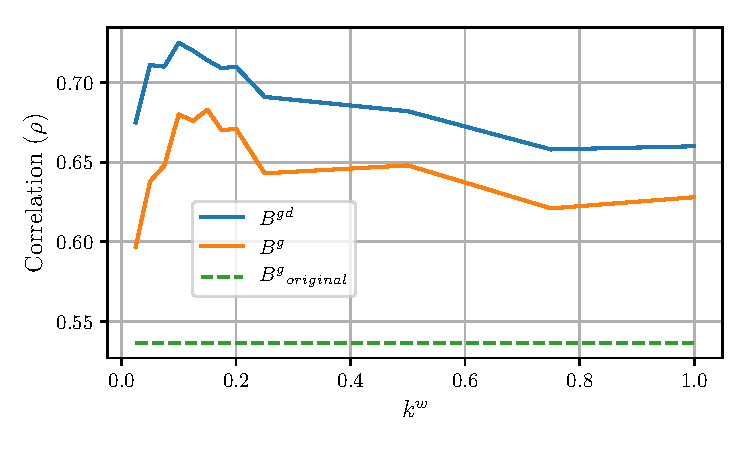
\includegraphics[width=8.0cm]{Figures/gender_correlation.pdf}
	\caption{Correlation of the \proposedmethod{} gender
          dimension with human judgments (blue) and the gender
          vector
          $w_{she} - w_{he}$ (orange) as a function of
          $k^w$. See Eqs.\ \ref{eq:bgd} / \ref{eq:bg}.
          Green dashed line: correlation of the original word2vec
          embeddings with the gender vector.}
	\label{fig:corr}
\end{figure}

        Figure \ref{fig:bias}
shows direct bias
          ($b^{direct}_1$, see Eq.\ \ref{eq:direct_bias})
of word2vec and \proposedmethod{}.
Naturally, imparting  a single
dimension with
gender information 
does not alter the overall bias in the word
 embeddings, but rather concentrates most of the bias on a
 single dimension as implied by Figure
 \ref{fig:corr}. Removing this dimension from the embedding
 space then considerably reduces the bias, especially for
 larger $k^w$. Figure \ref{fig:bias} also shows 
 $b^{direct}_1$
after debiasing.
$b^{direct}_1$
of the full and reduced imparted models (red dashed
 and dotted lines) are closer in this case, and
 substantially lower than that of word2vec. These results show that learning
   an embedding space with an explicit gender dimension
   enhances the performance of hard debiasing.

\begin{figure}
	\centering
	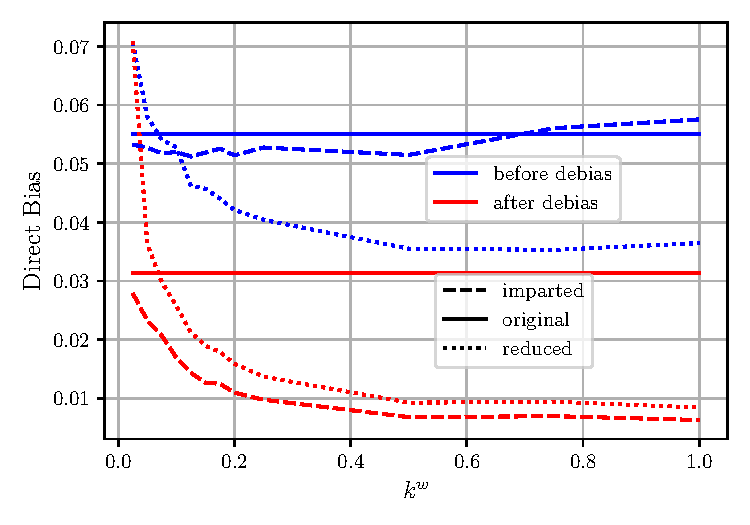
\includegraphics[width=8.0cm]{Figures/gender_bias_reduction.pdf}
	\caption{Direct bias
          ($b^{direct}_1$, see Eq.\ \ref{eq:direct_bias})
of the \proposedmethod{}
          (dashed lines) and reduced 
          (dotted lines) embeddings as a function of $k^w$. Solid lines:
          $b^{direct}_1$
 of the original embeddings. Blue/red: Results before/after
 hard debiasing.}
	\label{fig:bias}
\end{figure}

\subsubsection{Bias in Classification}

\citet{prost19biasTextClassif} give evidence that hard debiasing  introduces elevated
gender bias in high-level classification tasks when compared
with the original embedding model.
We therefore also use 
\textit{strong debiasing} \citep{prost19biasTextClassif},
a method that alleviates this issue
by taking $N$ (Eq.\ \eqref{eq:direct_bias}) as the entire
vocabulary as opposed to just gender neutral words.
As a baseline, we use \emph{scrubbing}
\citep{de19biosbias}, a technique that removes words characterized as
explicit gender indicators from the biographies prior to
classification.

Table \ref{tab:biosbias} compares
original embeddings, scrubbing, hard debiasing, strong
debiasing and the combination of \proposedmethod{} and
strong debiasing (B+S) on accuracy
(to measure task performance)
and TPR/TNR (Eq.\ \ref{eq:TPR}, to measure classification fairness).
The dataset is BiosBias.
Hard debiasing
has relatively high TPR/TNR, suggesting it
reduces classification fairness.
Strong debiasing 
on  original word2vec results in a relatively limited
change in classification fairness. Yet when
\proposedmethod{} and
strong debiasing are combined
(B+S),
$\text{TPR}_{\text{gap}}$ and $\text{TNR}_{\text{gap}}$
are lowered almost to the level of scrubbing,
without a major compromise in accuracy. These results
provide further evidence that concentration of gender
information on an embedding dimension improves performance
of debiasing methods.

\begin{table}
    \centering
	\begin{tabular}{lccc}
	    \hline \hline
        \textbf{Embedding} & \textbf{Acc.} & $\textbf{TPR}_{\textbf{gap}}$ & $\textbf{TNR}_{\textbf{gap}}$ \\\hline \hline %\hhline{===}
        word2vec & .717 & .094 & .0034 \\
        scrubbed & .717 & .061 & .0022 \\
        hard debiasing & .700 & .105 & .0037 \\
        strong debiasing & .699 & .087 & .0033 \\
        B+S$_{k^w=.1}$ & .697 & .066 & .0022 \\
        B+S$_{k^w=.5}$ & .699 & .067 & .0024 \\
        \hline \hline
	\end{tabular}
	\caption{Accuracy and True Positive/Negative Rate
          (TPR/TNR) on the occupation classification
          task. B+S = \proposedmethod{}+strong debiasing.}
	\label{tab:biosbias}
\end{table}

\enote{hs}{it's unusual to have  a very long
  conclusion. that's why i shortened it a lot}


\section{Conclusion} \label{sec:concl}

In this study, we introduced \proposedmethod{}, a new method for enhancing
interpretability of word embeddings by bidirectional
imparting of concepts extracted from lexical resources. 
%proposed method was implemented for the scalable word2vec
%algorithm, and semantic concepts were extracted from Roget's
%Thesaurus and WordNet.
In contrast to prior work, \proposedmethod{}
uses  both directions along each
dimension of the vector space separately, enabling encoding
of two different concepts; the two concepts can be chosen arbitrarily
or chosen as opposite concepts as a special case.  As a
result,
\proposedmethod{}
 makes more efficient use of
the embedding space while increasing encoding flexibility.

\enote{hs}{too much detail for conclusion?
  
The relative weighting of the interpretability objective
against the original word2vec objective was controlled by a
tunable parameter $k^w$. Evaluations on word analogy and
similarity tests suggest that limiting $k^w$ to a relatively
small range ($<0.2$) allows imparted models to attain on par
performance with the original embeddings.

}

We showed that  \proposedmethod{}
achieves higher interpretability of word embeddings copmared to
state-of-the-art methods, particularly in the negative
direction. At the same time, evaluation on word
similarity/analogy tests as well as sentiment, news and
question classification  showed that \proposedmethod{} does
not sacrifice task performance.
Thus, \proposedmethod{} offers a favorable
trade-off between the goals of enhancing
interpretability and maintaining task performance.


%on high-level natural language processing tasks. 

% An important advantage of the imparting method is its ability to concentrate information regarding a desired concept to a pre-defined embedding dimension. Specifically, 

\proposedmethod{} represents opposite concepts in a single
dimension on a continuum. As an important demonstration, we
used \proposedmethod{} to concentrate gender information in
a single gender dimension.  We showed that this gender
dimension has a high correlation with stereotypical gender
bias as measured by human judgments. Furthermore, we showed
that this gender dimension is useful for reducing gender
bias when coupled with debiasing.  The combination of
\proposedmethod{} and debiasing achieved lower levels of
gender bias and improved classification fairness. These
results highlight the potential of \proposedmethod{} in
reducing biases and stereotypes present in word embeddings.

% Here, the imparting method was demonstrated to improve interpretability and reduce gender bias in word2vec embedding models, using concepts from two common lexical sources. That said, imparting through modification of the learning objective is easily adaptable to different embedding algorithms, and to different lexical resources. The imparting framework can also be adopted for goals beyond interpretability enhancement, such as improvement of task performance. If imparting is used to encode task-relevant concepts, similar task performance can be achieved using simpler models with fewer dimensions. In turn, this can offer benefits in terms of memory requirements and computational load. 

\bibliography{NLP_MasterArchive}
\bibliographystyle{acl_natbib}


\clearpage

\appendix

\section{Appendices}



\subsection{Lexical Resources} 
\label{app:lexical_resources}

\begin{table*}
    \centering
	\begin{tabular}{lcccc}
	    \hline \hline
         \multirow{2}{*}{\textbf{Word Counts}} & \multicolumn{2}{c}{\textbf{Roget's Thesarus}}  & \multicolumn{2}{c}{\textbf{WordNet}} \\
         & \textbf{(300 grp.)} & \textbf{(600 grp.)} & \textbf{(300 grp.)} & \textbf{(600 grp.)} \\ \hline \hline %\hhline{====}
         Total & 20978 & 40350 & 26964 & 18965 \\ 
         Unique & 12289 & 19870 & 18123 & 13853 \\
         Average & 69.9$\pm$53.7 & 67.3$\pm$54.6 & 89.9$\pm$74.2 & 31.6$\pm$15.9 \\ \hline \hline %\hhline{====} 
	\end{tabular}
	\caption{Summary statistics of the word-group datasets}
	\label{tab:roget_vs_wordnet}
\end{table*}

In \citet{senel20impart}, Roget's Thesaurus \citep{Roget2008thesaurus} was designated as an external resource.
Here, in addition to Roget's Thesaurus, we also investigate  WordNet \citep{miller95wordnet} to extract semantic word-groups.
In order to extract a specific number of word-groups from WordNet, we partitioned the hierarchical structure starting from the root node, similar to the approach followed in \citet{senel20impart} for Roget's Thesaurus. We followed an iterative approach, where the largest node was divided to its hyponyms in each iteration. Node size was taken as the number of unique words descending from a node after filtering based on the vocabulary extracted from Wikipedia. We discarded the nodes with size less than $\lambda_{min}^w$. Iterations were stopped when the number of nodes exceeded the desired word-group count. Note that the desired word-group count may not be achieved if $\lambda_{min}^w$ is selected too large.
The groups with the smallest number of member words are discarded to achieve desired word-group.

We take $\lambda_{min}^w = 25$ and $\lambda_{min}^w = 15$ for 300 and 600 WordNet word groups, respectively.
Table \ref{tab:roget_vs_wordnet} summarizes the statistics for the constructed word-groups. 

% Please note that our method uses external resources only to select category labels which will be designated as the separate dimensions of the word embedding space. There is no explicit use of knowledge regarding similarity of words that belong each selected category.








\subsection{Training Parameters}
\label{app:training_parameters}

 For the training all imparted models and the original word2vec model, we used \verb|VOCAB_MIN_COUNT| $=100$, \verb|MAX_ITER| $=15$, \verb|WINDOW_SIZE| $=8$, \verb|NEGATIVE| $=15$, \verb|SAMPLE| $=10^{-4}$.
 
 
 
 
 
 
 
 \subsection{Comparison of Imparted Embeddings}
\label{app:impart_comparison}


\begin{figure*}
	\centering
	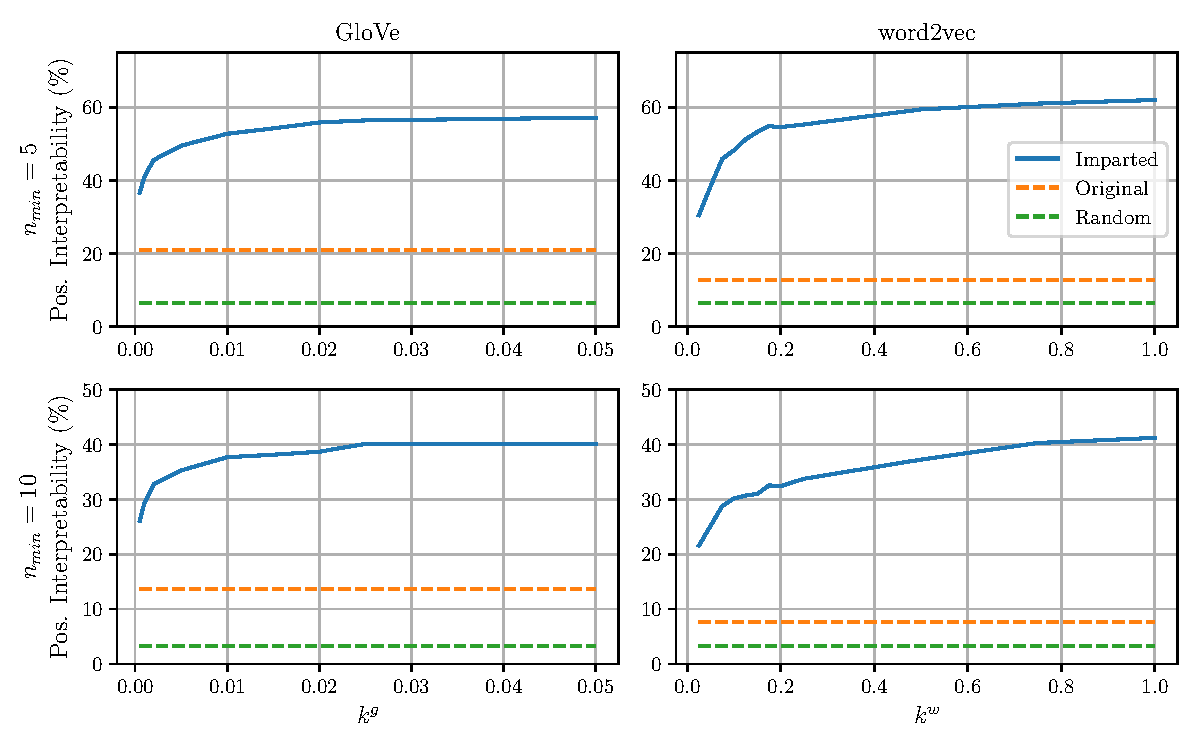
\includegraphics[width=16cm]{Figures/interpretability_glove_vs_word2vec.pdf}
	\caption{Interpretability scores in the positive direction $(IS^+)$ using $n_{min}=5$ (top row) and $n_{min}=10$ (bottom row) for unidirectionally imparted GloVe (left column) and word2vec (right column) algorithms for $k^g \in [0.0005,0.05]$ and $k^w \in [0.025,1.00]$, respectively. Interpretability scores for original embeddings and a random baseline are displayed for comparison as orange and green dashed lines, respectively.}
	\label{fig:g_vs_w2v}
\end{figure*}

Figure \ref{fig:g_vs_w2v} presents the interpretability levels of the unidirectionally imparted GloVe ($k^g \in [0.0005,0.05]$) and word2vec ($k^w \in [0.025,1.00]$) embeddings for $n_{min} = 5$ and $n_{min} = 10$, along with original embeddings and a random baseline. We can see that for both algorithms, imparting substantially improves interpretability. While interpretability of the imparted GloVe embedding does not increase for $k^g$ values beyond 0.03, that for the imparted word2vec embedding is gradually enhanced up to $k^w=1$. Note that the original word2vec embedding has relatively limited interpretability compared to the GloVe embedding.
Yet, for larger $k^w$, interpretability level of the imparted word2vec embedding improves, even surpassing GloVe. 
%These results indicate the viability of the imparting method for the online word2vec algorithm in order to improve interpretability in a memory-efficient and scalable setting.

% \begin{SCfigure*}
\begin{figure*}
	\centering
	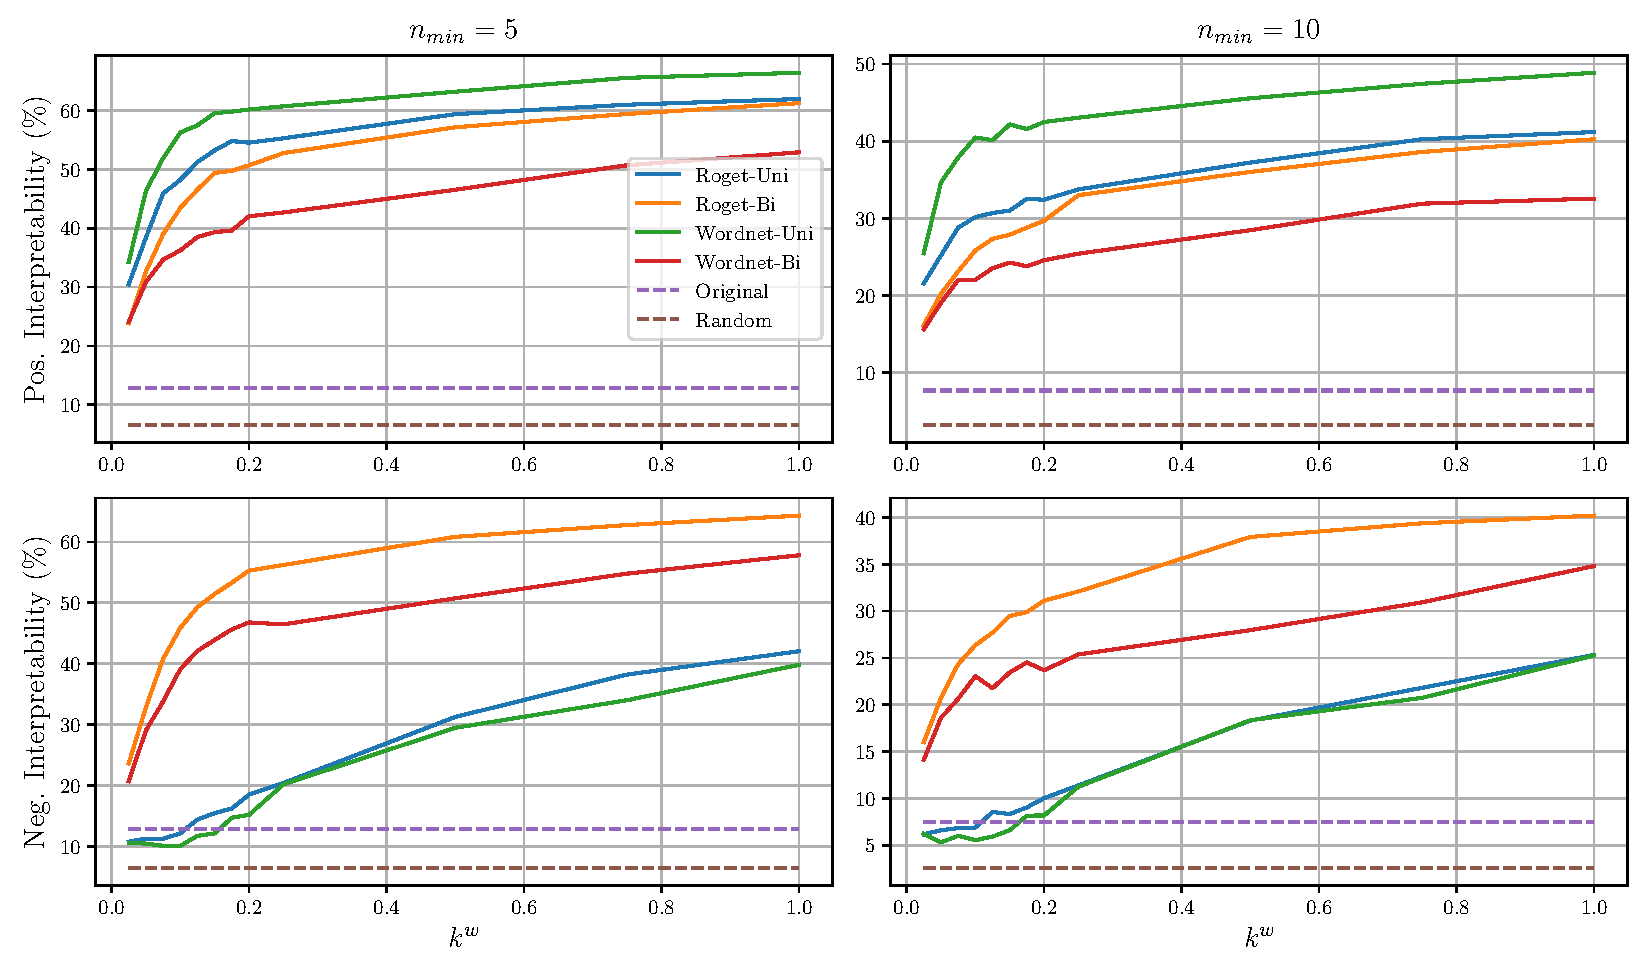
\includegraphics[width=16cm]{Figures/interpretability_wordnet_vs_roget.pdf}
	\caption{Positive (top) and negative (bottom)
          direction interpretability scores for
          unidirectionally imparted word2vec embeddings
          using Roget's Thesaurus (Roget-Uni) and WordNet
          (WordNet-Uni) and their bidirectionally imparted
          versions (\proposedmethod{} (Roget), \proposedmethod{} (WordNet)) for $k^w \in [0.025,1.00]$ along with the original word2vec embedding and a random baseline for $n_{min} = 5$ (left) and $n_{min} = 10$ (right).}
	\label{fig:wordnet_vs_roget}
\end{figure*}
% \end{SCfigure*}

% \begin{SCfigure*}
\begin{figure*}
	\centering
	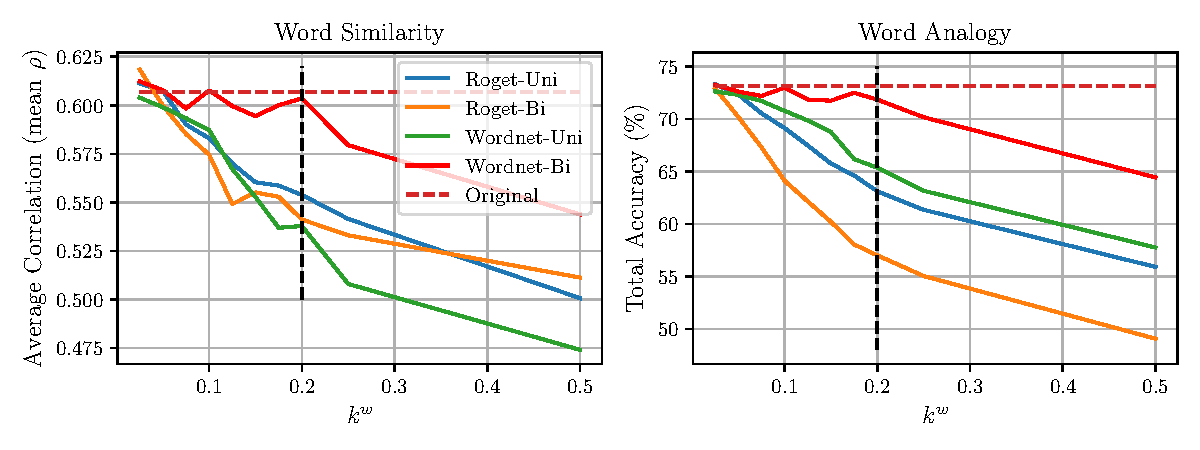
\includegraphics[width=16cm]{Figures/similarity_and_analogy.pdf}
	\caption{Performance of unidirectionally imparted word2vec embeddings using Roget's Thesaurus (Roget-Uni) and WordNet (WordNet-Uni) and their bidirectionally imparted versions (Roget-Bi, WordNet-Bi) for $k^w \in [0.025, 0.500]$ along with the original word2vec embedding on word similarity (left) and word analogy (right) tests. Word similarity results are presented as the average correlations from 13 different word similarity test sets.}
	\label{fig:sim_and_analogy}
\end{figure*}
% \end{SCfigure*}

Figure \ref{fig:wordnet_vs_roget} shows interpretability values of the imparted embeddings for $n_{min} = 5$ and $n_{min} = 10$ \textcolor{black}{in both of the positive and negative directions. It can be seen that bidirectional imparting achieves significantly improved interpretability compared to unidirectional imparting in the negative direction with minimal compromise in the positive direction.}

% Imparting improves interpretability in a controllable manner by offering a tuning parameter $k^w$, that adjusts how heavily the optimization objective weights interpretability against the original goal of capturing semantic relations among words. Naturally, emphasis on interpretability for relatively large values of $k^w$ might lead to suboptimal representation of word semantics. In order to investigate this, we evaluated the imparted embeddings on the intrinsic word analogy \citep{mikolov13word2vec_b} and word similarity \citep{faruqui14communityEval} tests. For analogy tests we use Google analogy dataset\footnote{http://download.tensorflow.org/data/questions-words.txt}. For brevity, word similarity results were averaged across 13 datasets\footnote{Word similarity datasets are: WS-353-ALL, SIMLEX-999, VERB-143, SimVerb-3500, WS-353-REL, RW-STANFORD, YP-130, MEN-TR-3k, RG-65, MTurk-771, WS-353-SIM, MC-30, MTurk-287} on which the evaluations were performed.

Figure \ref{fig:sim_and_analogy} presents the performances of the embeddings on word similarity and word analogy tests. It can be observed that performance on word similarity and analogy tests decreases with increasing $k^w$.  However, for bidirectional imparting of WordNet word-groups, performance is on par with original embeddings for $k^w \leq 0.2$. Taken together, results in Figs. \ref{fig:wordnet_vs_roget} and \ref{fig:sim_and_analogy} suggest that bidirectional imparting of WordNet word-groups at relatively low $k_w$ is the optimal setting for word2vec. While WordNet word-groups somewhat reduce interpretability compared to Roget word-groups in bidirectional setting, they are much better at preserving the semantic structure of the embedding space as suggested by similarity and analogy tests.
 
 
 
 
 
 
 
 
 \subsection{Competing Methods}
 \label{app:competing_methods}
 
 OIWE-IPG was trained on the same corpus as the word2vec embeddings using the default parameters reported in \citep{luo15online} \textcolor{black}{, yielding 300 dimensional vectors}. SOV and Parsimax that work on pretrained embeddings were performed on the original word2vec embeddings, again using suggested parameters in \citep{faruqui15sparse} and \citep{park17rotated}, \textcolor{black}{resulting in 1000 and 300 dimensional vectors, respectively.} For Word2Sense, we used the publicly available \textcolor{black}{2250 dimensional} pretrained vectors\footnote{https://github.com/abhishekpanigrahi1996/Word2Sense} due to computational restrictions. \textcolor{black}{For POLAR, we trained two different versions. First, we obtained 1465 dimensional POLAR-large embeddings that were reported in \citep{mathew20polar}, by applying polar transformation on Google's pretrained word2vec embeddings\footnote{https://drive.google.com/file/d/0B7XkCwpI5KDYNlNUTTlSS21pQmM} using all 1465 antonym pairs. Note that these embeddings were originally trained on a much larger corpus (Google News) with a substantially larger vocabulary (3 million) than our word2vec embeddings. Therefore, POLAR-large embeddings are significantly more expensive than our imparted embeddings in terms of computational and linguistic resources. Second, we obtained 500 dimensional POLAR-small embeddings that are more comparable to imparted embeddings in terms of model dimensionality and resource usage, by performing the polar transformation on our original word2vec embeddings using the default parameters\footnote{https://github.com/Sandipan99/POLAR}.} 
 
 
 
 
 
 
 

\subsection{Classification Tasks}
\label{app:clf_tasks}

The classification tasks are described in detail below:
\begin{itemize}
    \item \textbf{Sentiment Analysis:} A sentence-level binary classification task using the Stanford Sentiment Treebank consisting of thousands of movie reviews \citep{socher13treebank} and their sentiment scores. The development and training sets in the original dataset were aggregated, and reviews with neutral scores were removed (i.e., scores between 0.4 and 0.6). The resulting dataset contained 7407 training and 1751 test samples.
    
    \item \textbf{Question Classification (TREC):} A question-level multinomial classification task using the TREC dataset \citep{li06learning} consisting of six different types of questions (person, location, entity, number, description, abbreviation). This dataset consisted of 5452 training and 500 test questions.
    
    \item \textbf{News Classification:} Following \citep{faruqui15sparse}, three news-level binary classification tasks were considered using the 20 Newsgroup dataset\footnote{http://qwone.com/~jason/20Newsgroups}. The following news topics were considered (training/test sample counts): 1) Religion: atheism vs christian (1079/716); 2) Sports: baseball vs hockey (1192/796); 3) Computers: IBM vs Mac (1162/775).
\end{itemize}

For these high-level NLP tasks, we took the average of the word vectors in input text (can be a sentence, question or news) as input features and trained an SVM classifier that was tuned using 5 fold cross-validation on the training sets. 






\subsection{Performance of Gender Biased Embeddings}

A potential risk of debiasing on gender-imparted models is undesirable loss of semantic structure in the embedding space that might compromise task performance. To rule out this risk, we evaluated the embeddings in the gender-bias experiments on intrinsic tests and downstream classification tasks. For the imparted and reduced embeddings, we averaged the results across $k^w$. Table \ref{tab:gender_performance_tests} shows that all the evaluated embeddings perform nearly as good as the original embeddings on all tasks, except a slightly reduced performance on computer news classification task. These results indicate that debiasing of gender-imparted embeddings successfully preserves semantic structure of the embedding space.

\begin{table*}
    \centering
	\begin{tabular}{lcccccc}
		\hline \hline 
		\multirow{2}{*}{\textbf{Task}} & \multicolumn{3}{c}{\textbf{before debias}} & 
		\multicolumn{3}{c}{\textbf{after debias}} \\
		 & \textbf{word2vec} & \textbf{imparted} & \textbf{reduced} & \textbf{word2vec} & \textbf{imparted} & \textbf{reduced} \\ \hline \hline %\hhline{======}
	    Sem. Anlg. & 79.87 & 79.00 $\pm$ 0.50 & 79.16 $\pm$ 0.50 & 78.65 & 78.92 $\pm$ 0.57 & 78.99 $\pm$ 0.61 \\
	    Syn. Anlg. & 67.63 & 66.39 $\pm$ 0.99 & 66.48 $\pm$ 1.01 & 67.46 & 66.42 $\pm$ 0.96 & 66.43 $\pm$ 1.00 \\ 
	    \hline %\hhline{------}
	    Word Sim. & 60.68 & 60.08 $\pm$ 0.66 & 60.21 $\pm$ 0.52 & 60.64 & 60.12 $\pm$ 0.67 & 60.28 $\pm$ 0.53 \\
	    \hline %\hhline{------}
	    Sent. Anly. & 80.30 & 79.95 $\pm$ 0.36 & 79.94 $\pm$ 0.33 & 79.84 & 79.99 $\pm$ 0.37 & 79.98 $\pm$ 0.41 \\ \hline %\hhline{------}
	    Quest. Clf. & 85.80 & 84.63 $\pm$ 0.59 & 86.00 $\pm$ 0.92 & 86.20 & 86.27 $\pm$ 0.74 & 86.03 $\pm$ 0.80 \\ \hline %\hhline{------}
	    Sports News & 95.85 & 95.33 $\pm$ 0.27 & 95.34 $\pm$ 0.25 & 95.10 & 95.33 $\pm$ 0.27 & 95.33 $\pm$ 0.29 \\
	    Relig. News & 87.01 & 86.19 $\pm$ 0.61 & 86.10 $\pm$ 0.57 & 86.03 & 86.24 $\pm$ 0.59 & 86.18 $\pm$ 0.59 \\
	    Comp. News & 81.55 & 78.74 $\pm$ 0.84 & 78.73 $\pm$ 0.99 & 78.84 & 78.68 $\pm$ 0.83 & 78.63 $\pm$ 0.81 \\ \hline \hline %\hhline{======}
	\end{tabular}
	\caption{Results of embeddings from gender bias experiments on the performance evaluation tests. }
	\label{tab:gender_performance_tests}
\end{table*}








\subsection{Hybrid Gender and Interpretability Imparted Embeddings}

\begin{table}
    \centering
	\begin{tabular}{lccc}
		\hline \hline 
		\textbf{Task} & \textbf{$\setlength{\thickmuskip}{0mu}k^w=0.1$} & \textbf{$\setlength{\thickmuskip}{0mu}k^w=0.2$} & \textbf{$\setlength{\thickmuskip}{0mu}k^w=1$}\\ \hline \hline %\hhline{======}
	    Semantic Anlg. & 79.07 & 78.13 & 73.25 \\
	    Syntactic Anlg. & 66.61 & 65.17 & 45.58 \\ 
	    \hline %\hhline{------}
	    Word Sim. & 60.62 & 59.11 & 48.94 \\
	    \hline %\hhline{------}
	    Sentiment Anly. & 80.41 & 79.55 & 79.84 \\ \hline %\hhline{------}
	    Question Clf. & 84.60 & 85.00 & 84.20 \\ \hline %\hhline{------}
	    Sports News & 96.11 & 95.73 & 95.73 \\
	    Religion News & 85.89 & 87.43 & 88.55 \\
	    Comput. News & 81.42 & 81.03 & 79.74 \\\hline
	    Interp.$^+_{n_{min}=5}$ & 36.88 & 41.22 & 54.28 \\
	    Interp.$^-_{n_{min}=5}$ & 38.47 & 44.79 & 58.50 \\
	    Interp$^+_{n_{min}=10}$ & 22.41 & 24.17 & 34.07 \\
	    Interp.$^-_{n_{min}=10}$ & 22.49 & 23.89 & 35.43 \\\hline
	    Gender B.$_{reduced}$ & 0.0470 & 0.0403 & 0.0441 \\
	    Gender B.$_{debiased}$ & 0.0168 & 0.0122 & 0.0148 \\ 

	    \hline \hline %\hhline{======}
	\end{tabular}
	\caption{ Results of Evaluation Tests for the Hybrid Gender and Interpretability Imparted Embeddings.}
	\label{tab:gender_plus_wordnet}	
\end{table}

Finally, we demonstrated the feasibility of the proposed approach for concurrent gender and interpretability imparting. To do this, we obtained a hybrid model where the first dimension was encoded with gender word-groups and the remaining 299 dimensions were bidirectionally imparted with word-groups extracted from WordNet. Evaluation on gender bias, interpretability and task performance were repeated on this hybrid model. We find that the hybrid embeddings perform similarly to WordNet-Bi in terms of interpretability and task performance, for all evaluations and for all $k^w$ (Table \ref{tab:gender_plus_wordnet}). We also find that the hybrid embeddings perform similarly to gender-imparted embeddings in gender bias evaluations (Table \ref{tab:gender_plus_wordnet}). These results indicate that the proposed bidirectional imparting method enables gender debiasing and interpretability enhancement simultaneously in embedding models without compromising task performance.

\end{document}
